\documentclass[12pt]{article}

\usepackage[margin=1in]{geometry}
\usepackage[pdftex]{hyperref}
\usepackage{amsmath,amsthm,amssymb,graphicx,mathtools,tikz,hyperref,enumerate}
\usepackage{mdframed,cleveref,cancel,stackengine,pgfplots,mathrsfs,physics}

\newmdenv[leftline=false,topline=false]{topright}
\let\proof\relax
\usepackage[utf8]{inputenc}
\usetikzlibrary{positioning}
\newcommand{\n}{\mathbb{N}}
\newcommand{\z}{\mathbb{Z}}
\newcommand{\q}{\mathbb{Q}}
\newcommand{\cx}{\mathbb{C}}
%\newcommand{\real}{\mathbb{R}}
\newcommand{\E}{\mathbb{E}}
\newcommand{\F}{\mathbb{F}}
\newcommand{\h}{\mathscr{H}}
\newcommand{\bb}[1]{\mathbb{#1}}
\let\k\relax
\newcommand{\k}{\mathbf{k}}
\newcommand{\ita}[1]{\textit{#1}}
\newcommand\inv[1]{#1^{-1}}
\newcommand\setb[1]{\left\{#1\right\}}
\newcommand{\vbrack}[1]{\langle #1\rangle}
%\newcommand{\determinant}[1]{\begin{vmatrix}#1\end{vmatrix}}
%\newcommand{\abs}[1]{\left\vert #1 \right\vert}
\newcommand{\Po}{\mathbb{P}}
\DeclareMathOperator{\Id}{Id}
\DeclareMathOperator{\rg}{rg}
\DeclareMathOperator{\car}{car}


\hypersetup{
	colorlinks=true,
	linkcolor=blue,
}

\newtheoremstyle{break}% name
{}%         Space above, empty = `usual value'
{}%         Space below
{}% Body font
{}%         Indent amount (empty = no indent, \parindent = para indent)
{\bfseries}% Thm head font
{}%        Punctuation after thm head
{\newline}% Space after thm head: \newline = linebreak
{#1 #2 \normalfont #3}%         Thm head spec


\theoremstyle{break}
\newtheorem{ej}{Ejercicio}
\let\proof\relax
\newtheorem*{proof}{Demostración}

\renewcommand{\thesection}{\Alph{section}.}

\usetikzlibrary{decorations.fractals}
\pgfplotsset{compat=1.15}

\begin{document}
\date{

\title{Topologia}
\author{Ernesto Lanchares}
\maketitle

\section{El teorema de contracción de Banach}

Una \emph{contracció} de constant $0 \leq c < 1$ és una aplicació $f \colon X \to X$ tal que
\[
	d\left( f(x), f(y) \right) \leq c \cdot d(x, y), \qquad \forall x, y \in X.
\]
\begin{enumerate}[a)]
\item\label{item:con} Proveu que tota contracció es contínua.

	Vamos a demostrarlo por la definición $\varepsilon$-$\delta$ de continuidad.
	Dado un $\varepsilon$, $\exists \delta = \frac{\varepsilon}{c}$ tal que
	\[
		d(x, y) < \delta \implies d\left( f(x), f(y) \right) \leq c d(x,y) < c\frac{\varepsilon}{c} = \varepsilon
	\].
\item\label{item:otra} Proveu que, per a qualsevol $z \in X$, la succesió $\setb{f^n(z)}$ és de Cauchy.

	Se tiene que
	\[
		\begin{aligned}
			d\left( f^n(z), f^{n+m}(z) \right) &\leq cd\left( f^{n-1}(z), f^{n+m-1}(z) \right) \\
			& \quad \vdots \\
			&\leq c^n d\left(z, f^m(z) \right)
		\end{aligned}
	\]

	Ahora, nos resta acotar $d\left( z, f^m(z) \right)$. Para ello, tomamos
	\[
		\begin{aligned}
			d\left( z, f^{m+1}(z) \right) &\leq d\left( z, f^m(z) \right) + d\left( f^m(z), f^{m+1}(z) \right) \\
			&\leq d\left( z, f^m(z) \right) + c^m d\left( z, f(z) \right)
		\end{aligned}
	\]
	Por lo tanto, se cumple la siguiente desigualdad
	\[
		d\left( z, f^m(z) \right) \leq \left( \sum^m_{i = 0} c^i \right) d\left( z, f(z) \right) \leq
		\frac{1}{1-c} d\left( z, f(z) \right)
	\]
	Con lo cual, dado un $\varepsilon > 0$, $\exists N$ tal que
	\[
		n > N \implies c^n \leq \frac{1-c}{d\left( z, f(z) \right)}\varepsilon
	\]
	Y, por lo tanto,
	\[
		d\left( f^n(z), f^{n+m}(z) \right) \leq c^nd\left( z, f^m(z) \right)
		\leq c^n \frac{d\left( z, f(z) \right)}{1 - c} \leq \varepsilon
	\]
	Es decir, que $\setb{f^n(z)}_{n \in \n}$ es de Cauchy.

\item\label{item:teob} \emph{Teorema de contracció de Banach}: proveu que tota contracció de $X$ té un únic punt fix.
	És a dir, existeix un únic $x \in X$ tal que $f(x) = x$.

	Como $X$ es un espacio métrico completo, que una sucesión sea de Cauchy implica que es convergente,
	por lo tanto $\exists p = \lim\limits_{n \to \infty} f^n(z)$. Y se tiene que 
	\[
		f(p) = f\left( \lim_{n \to \infty} f^n(z) \right) \stackrel{(f \text{ continua})}{=} \lim_{n \to \infty} f^{n+1}(z) = p
	\]

	Veremos ahora que es único. Suponemos que $x$ e $y$ son dos puntos fijos por $f$ tales que $x \neq y$,
	por lo tanto, $d(x, y) > 0$, entonces
	\[
		d(x, y) < c d\left( f(x), f(y) \right) = c d(x, y) \implies 1 < c
	\]
	Lo cual nos lleva a una contradicción, y por lo tanto $x = y$.
\end{enumerate}

\section{L’hiperespai de Hausdorff dels subespais compactes.}
Definim
\[
	\h(X) = \setb{A \subset X \vert A \text{ compacto}}
\]

\begin{enumerate}[a)] \setcounter{enumi}{3}
\item Observeu que la definició ordinària de distàcia $d(A,B)$
	entre dos conjunts $A, B \in \h(X)$ no és una distància a
	$\h(X)$. Definim
	\[
		d_1(A, B) = \max_{a \in A} \setb{d(a, B)}, \quad d_2(A, B)
		= \max_{b \in B} \setb{d(A, b)}
	\]
	Calculeu $d_1$, $d_2$ en l'exemple següent: $X = \mathbb{R}^2$,
	$A = \setb{(x, y) \in \mathbb{S}^1 \vert y \geq 0}$ i
	$B = [-2, 2] \times \{2\}$. Deduïu que $d_1$, $d_2$ no són
	distàncies.


	Primero, calculamos $d_1(A, B)$. Para ello, tomamos un punto
	arbitrario $a \in A$ y maximizamos $d(a, B)$. Para calcular
	$d(a, B)$, tomamos un punto arbitrario de $B$ y minimizamos
	$d(a, b)$. Primero tomamos
	$(\cos \theta, \sin \theta) \in A$ y $(t, 2) \in B$ (con
	$\pi \leq \theta \leq 0$ y $-2 \leq t \leq 2$). y tenemos
	\[
		d^2(a, b) = \left( \cos \theta - t \right)^2 + \left( \sin
		\theta -2 \right)^2 \qquad \frac{\partial d^2(a,
		b)}{\partial t} = 2t - 2\cos \theta
	\]
	Por lo tanto, el mínimo se alcanza cuando $t = \cos \theta$,
	y en ese punto, el valor de $d$ es
	\[
		d^2(a, B) = \cancelto{0}{\left( \cos \theta - \cos \theta
		\right)^2} + \left( \sin \theta - 2 \right)^2
	\]
	Lo que quiere decir que
	\[
		d_1(A, B) = \max_{\theta \in [0, \pi]} \abs{\sin \theta -
		2}
	\]
	Por lo tanto, $d_1(A, B) = 2$.

	Pasamos ahora a calcular $d_2(A, B)$.
	\begin{gather*}
		d^2(a, b) = (\cos \theta - t)^2 + \left( \sin \theta - 2 \right)^2 \\
		\frac{\partial d^2(a, b)}{\partial \theta} =
		\cancel{-2\sin \theta \cos \theta} + 2t\sin \theta -
		\cancel{2\cos\theta\sin\theta} - 4 \cos \theta
	\end{gather*}
	Por lo tanto, el mínimo se alcanza cuando
	$t \sin \theta = 2 \cos \theta \implies \theta = \arctan
	\frac{2}{t}$. Substituyendo, obtenemos
	\[
		d^2(A, b) = \left( \cos \left( \arctan \frac{2}{t} \right)
		- t \right)^2 + \left( \sin \left( \arctan \frac{2}{t}
		\right) - 2 \right)^2 = \left( t
		\sqrt{\frac{t^2+4}{t^2}} - 1 \right)^2
	\]
	Ahora, derivamos para buscar el maximo, obteniendo
	\[
		\dv{d^2(A, b)}{t} = 2t - \frac{2 \abs{t}}{\sqrt{t^2+4}}
	\]
	Que no se anula en ningún punto. Con lo cual, el máximo se
	haya en un extremo con $t = 2$ (o $t = -2$) y se obtiene:
	\[
		d_2(A, B) = \left( \cos \frac{\pi}{4} - 2\right)^2 +
		\left( \sin \frac{\pi}{4} - 2 \right)^2 \approx 3.343
	\]
	Que coincide con la intuición geométrica que pudieramos
	tener:
	\begin{center}
		\begin{tikzpicture}
			\begin{axis}[width=\textwidth/1.5, axis equal, axis
				lines = center, xmin=-2, xmax=2, ticks=none]
				\addplot[color=blue,samples=100,domain=0:180]
				({cos(x)}, {sin(x)}); \addplot[color=red,domain=-2:2]
				{2};

				\addplot[color=orange,mark=*] coordinates { (-2, 2)
				(-0.70710678118654, 0.70710675118554) }
				node[above,pos=1] {$d_2$};
				\addplot[color=purple,mark=*] coordinates { (1, 2) (1,
				0) } node[above right,pos=1] {$d_1$};
			\end{axis}
		\end{tikzpicture}
	\end{center}
	Ya que $d_1(A,B) = d_2(B, A)$ (y viceversa), observamos que ni
	$d_1$ ni $d_2$ no cumplen la propiedad simétrica, y por lo
	tanto no son distancias.
\item Definim $h(A,B) = \max \setb{d_1(A, B), d_2(A,
	B)}$. Proveu que $\left( \h(X), h\right)$ és un espai
	mètric.  Asumirem que $\h(X)$ és un espai mètric
	\emph{complet}.
	\newpage
	Tenemos que demostrar que
	\begin{enumerate}[i)]
	\item $h(A,B) \geq 0$ y $h(A, B) = 0 \iff A = B$.

		Que $h \geq 0$ es trivial por la definición de $d_1$ y de
		$d_2$.

		Ahora, supondremos que $h(A, B) \neq 0$, entonces o bien
		$d_1(A, B) > 0$ o bien $d_2(A, B) > 0$, suponemos que es
		$d_1$ (el caso de $d_2$ es análogo). Entonces, existe
		$a \in A$ tal que
		$d_1(a, B) > 0 \implies a \notin B \implies A \neq B$.

		Ahora, supondremos que $A = B$, entonces
		$d(a, B) = d(b, A) = 0$, $\forall a \in A, b \in B$, y por
		lo tanto, $h(A, B) = d_1(A, B) = d_2(A, B) = 0$.
	\item $h(A, B) = h(B, A)$.

		Tenemos que
		\[
			h(A, B) = max \setb{d_1(A, B), d_2(A, B)} = \setb{d_2(B,
			A), d_1(B, A)} = h(B, A).
		\]
	\item $h(A, B) \leq h(A, C) + h(C, B)$.

		Ahora, veremos que $d_1(A, B) \leq d_1(A, C) + d_1(C, B)$,
		y análogamente $d_2(A, B) \leq d_2(A, C) + d_2(C, B)$.
		
		Para todo $a \in A$ se cumple que
		\[
			d(a, B) \leq d(a, c) + d(c, B)
		\]
		Donde $c$ es tal que
		$d(a, c) = \min\limits_{c \in C} \setb{d(a, c)}$ (que existe por ser $C$ compacto). Ya que
		si fuera falso, es decir $\exists b_1 \in B$ (por ser $B$ compacto) tal que
		\[
			d(a, B) = d(a, b_1) > d(a, c) + d(c, B)
		\]
		Entonces, existe $b_2 \in B$ tal que
		$d(c, b_2) = d(c, B)$ (de nuevo, por ser $B$ compacto). Y por lo tanto,
		\[
			d(a, B) = d(a, b_1) > d(a, c) + d(c, b_2) \stackrel{(*)}{>} d(a, c) +
			d(c, b_1)
		\]
		(*Por definición de distancia a un conjunto), Contradicción con la
		desigualdad triangular, por lo tanto, el resultado inicial
		es cierto. Y ahora, como se cumple $\forall a \in A$, se
		cumple para el máximo:
		\[
			\begin{aligned}
				d_1(A, B) &\leq d(a, c) + d(c, B) \\
				&\leq d(a, C) + d(c, B) \\
				&\leq d_1(A, C) + d(c, B) \\
				&\leq d_1(A, C) + d_1(C, B)
			\end{aligned}
		\]

		Una vez visto esto, se tiene que
		\[
			\begin{aligned}
				h(A, B) &= \max \setb{ d_1(A, B), d_2(A, B) } \\
				&\leq \max \setb{ d_1(A, C) + d_1(C, B), d_2(A, C) + d_2(C, B) } \\
				&\leq \max \setb{ d_1(A, C), d_2(A, C) } + \max \setb{ d_1(C, B), d_2(C, B) } \\
				&= h(A, C) + h(C, B)
			\end{aligned}
		\]
	\end{enumerate}
\item Proveu que tota contracció $f \colon X \to X$ s'estén a
	una contracció $f \colon \h(X) \to \h(X)$.

	\quad

	Primero, tenemos que asegurar que $f$ está bien definida, lo cual es inmediato por el apartado
	\ref{item:con} que nos asegura que $f$ es continua, y por lo tanto $f(A)$ ($A$ compacto) es compacto.

	Tomamos un punto cualquiera $a \in A$, y sea $b$ tal que
	$d(a, b) = d(a, B)$ (que existe por $B$ compacto), entonces
	\[
		d_1\left( f(a), f(B) \right) \leq \left( f(a), f(b) \right)
		\leq c \cdot d(a, b) = c \cdot d(a, B) \leq c \cdot d_1(A,
		B)
	\]
	Y cómo se cumple para todo $f(a)$, se cumple para el máximo,
	y se tiene
	\[
		d_1\left( f(A), f(B) \right) \leq c \cdot d_1(A, B)
	\]
	Ahora, se tiene
	\[
		\begin{aligned}
			c \cdot h(A, B) &= \max \setb{ c \cdot d_1(A, B), c \cdot d_2(A, B) } \\
			&\leq \max \setb{ d_1\left( f(A), f(B) \right), d_2\left( f(A), f(B) \right) } \\
			&= h\left( f(A), f(B) \right)
		\end{aligned}
	\]
\item Proveu que per a qualsevol $A, B, C, D \in \h(X)$
	se satisfà
	\[
		h\left( A \cup B, C \cup D \right) \leq \max \setb{ h(A,
		C), h(B, D) }.
	\]
	Apliqueu aquesta desigualtat per a deduir el teorema de
	contracció de $\h(X)$: Si $G_i \colon \h(X) \to \h(X)$,
	$1 \leq i \leq n$, són contraccions de constants $c_i$,
	aleshores $\Gamma \colon \h(X) \to \h(X)$ definida per
	\[
		\Gamma(A) = \bigcup_{1 \leq i \leq n} G_i(A)
	\]
	és una contracció de constant
	$c = \max \setb{ c_1, \dots, c_n }$.

	\quad

	Primero, demostraremos que
	\[
		d_1(A \cup B, C \cup D) \leq \max \setb{ d_1(A, C), d_1(B, D) }
	\]
	(y análogamente para $d_2$).
	\[
		\begin{aligned}
			d_1(A \cup B, C \cup D) &\leq \max \setb{ d_1(A, C \cup D), d_1(B, D \cup D) } \\
			&\leq \max \setb{ \min \setb{d_1(A, C), d_1(A, D)}, \min \setb{d_1(B, C), d_1(B, D)}} \\
			&\leq \max \setb{ d_1(A, C), d_1(B, D)}
		\end{aligned}
	\]
	Y análogamente para $d_2$. Ahora
	\[
		\begin{aligned}
			h(A \cup B, C \cup D) &= \max \setb{d_1(A \cup B, C \cup D), d_2(A \cup B, C \cup D)} \\
			&\leq \max \setb{\max \setb{d_1(A, C), d_1(B, D)}, \max \setb{d_2(A, C), d_2(B, D)}} \\
			&= \max \setb{ d_1(A, C), d_2(A, C), d_1(B, D), d_2(B, D)} \\
			&= \max \setb{ \max \setb{d_1(A, C), d_2(A, C)}, \max \setb{d_1(B, D), d_2(B, D)}} \\
			&= \max \setb{ h(A, C), h(B, D) }
		\end{aligned}
	\]

	Ahora, generalizamos el resultado por inducción. Acabmos de
	demostrar el paso base, suponemos ahora que se cumple para
	$n$, es decir,
	\[
		h(A_1 \cup \cdots \cup A_n, C_1 \cup \cdots C_n) \leq \max
		\setb{ h\left( A_1, C_1 \right), \dots, h\left( A_n, C_n
		\right)}
	\]
	Ahora
	\[
		\begin{aligned} 
			h\left( A_1 \cup \cdots \cup A_n \cup B, C_1 \cup \cdots
			\cup C_n \cup D \right) &\leq \max \setb{ h\left( A_1
					\cup \cdots \cup A_n, C_1 \cup \cdots \cup C_n
			\right), h(B, D)} \\ &\leq \max \setb{ h\left( A_1,
				C_1 \right), \dots, h\left( A_n, C_n \right), h(B,
			D)}
		\end{aligned}
	\]
	Por lo tanto el resultado se cumple para $n+1$ y el queda
	probado.

	Ahora, consideramos la $\Gamma$ del enunciado, entonces
	\[
		\begin{aligned}
			h\left( \Gamma(A), \Gamma(B) \right) =
			h\left( \bigcup_{1 \leq i \leq n} G_i(A), \bigcup_{1
			\leq i \leq n} G_i(B) \right)
			&\leq \max_{1 \leq i \leq n} \setb{ h\left( G_i(A), G_i(B) \right)} \\
			&\leq \max_{1 \leq i \leq n} \setb{ c_i h(A, B) } \\
			&\leq \max_{1 \leq i \leq n} \setb{ c_i } h(A, B)
		\end{aligned}
	\]
	Por lo tanto, $\Gamma$ es una contracción de constante $c = \max\limits_{1 \leq i \leq n} \setb{c_i}$.

\item Prenem $X = I$. Considerem les aplicacions
	$g_1, g_2 \colon I \to I$ definides per
	\[
		g_1(x) = x/3, \qquad g_2(x) = x/3 + 2/3.
	\]
	Determineu el compacte de $I$ que és el punt fix de la
	contracció $\Gamma(A) = g_1(A) \cup g_2(A)$.
	
	\quad

	Demostraremos que el compacto que es punto fijo de la
	contracción es el conjunto de Cantor ($C$), que se define de la
	siguiente forma:
	\[
		C = \setb{\left. \sum^\infty_{1 \leq i} \frac{2a_i}{3^i} \right\vert a_i \in \setb{0, 1} \quad \forall i \in \n}
	\]

	Ahora, veremos que $\Gamma(C) = C$, y por lo tanto, $C$ será el único punto fijo de la contracción. Para ello, nos será útil
	trabajar en ternario, ya que el conjunto $C$ consta de los números entre 0 y 1 que se pueden escribir con ceros y doses en base 3 
	(inmediato por la definición).

	Vamos a ver que $\Gamma(C) \subseteq C$. Tomamos $x \in C$, entonces
	\[
		\Gamma(x) = g_1(x) \cup g_2(x)
	\]
	Si $x = 0.d_1d_2d_3\cdots$, se tiene que
	\[
		g_1(x) = 0.0d_1d_2d_3\cdots \qquad g_2(x) = 0.2d_1d_2d_3\cdots
	\]
	(en base 3). Tanto $g_1(x)$ como $g_2(x)$ son números entre 0 y 1 que se pueden escribir con ceros y doses, por lo tanto $x \in C$.

	Ahora comprobaremos que $C \subseteq \Gamma(C)$. Tomamos $x = (0.d_1d_2d_3\cdots) \in C$, entonces
	\[
		x \in \Gamma(0.d_2d_3\cdots)
	\]
	Si $d_1 = 0$, efectivamente $x = g_1(0.d_2d_3\cdots)$. Y si $d_1 = 2$, entonces $x = g_2(0.d_2d_3\cdots)$. Y efectivamente,
	$(0.d_2d_3\cdots) \in C$.

	Ahora, resta ver que $C$ es compacto. Para ello, nos resultará útil otra caracterización constructiva de conjunto de cantor
	de forma geométrica. Esta caracterización es de carácter recursivo y en cada paso elimina el segmento abierto correspondiente
	al tercio central de cada intervalo.

	Geométricamente obtenemos la siguiente figura:
	\begin{center}
		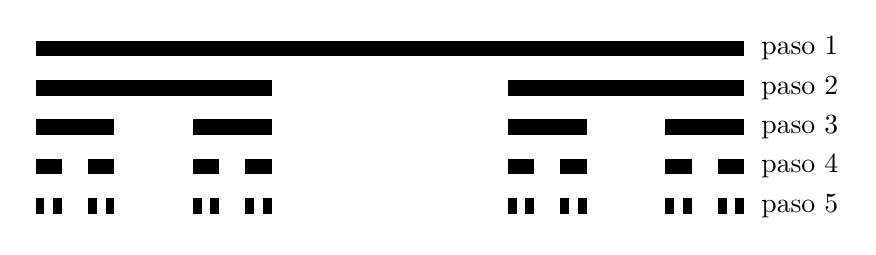
\begin{tikzpicture}[decoration=Cantor set,line width=2mm]
			\draw (0,0) -- (9,0) node [right]  {paso 1};
			\draw decorate{ (0,-.5) -- (9,-.5)} node [right] {paso 2};
			\draw decorate{ decorate{ (0,-1) -- (9,-1) }} node [right] {paso 3};
			\draw decorate{ decorate{ decorate{ (0,-1.5) -- (9,-1.5) }}} node [right] {paso 4};
			\draw decorate{ decorate{ decorate{ decorate{ (0,-2) -- (9,-2) }}}} node [right] {paso 5};
		\end{tikzpicture}
	\end{center}
	Es fácil ver que en el paso 1, tenemos los números en ternario entre 0 y 1. En el paso 2, aquellos cuyo primer
	dígito es un 0 o un 2. En el paso 3, aquellos cuyos primeros 2 dígitos son ceros o doses, y, en general, en el paso
	$n$, tendremos aqeullos números en ternario cuyos $n-1$ primeros dígitos son o ceros o doses.

	Por lo tanto, al llevar esta construcción al infinito, obtenemos el conjunto de Cantor. Ahora, es fácil ver que este conjunto
	es compacto. Ya que es claramente acotado, y cerrado (por ser complementario de la unión de todos los abiertos que vamos retirando) y
	por lo tanto, en la topología de $I$, es un compacto.
\end{enumerate}
\end{document}

